\documentclass{tufte-handout}
\usepackage{amsmath}
\usepackage{siunitx}
\usepackage{physics}
\usepackage{nicefrac}
\usepackage{unicode-math}
\usepackage{tikz}
\usetikzlibrary{matrix, arrows}

\definecolor{nicered}{HTML}{661F25}
\definecolor{nicegreen}{HTML}{1F663C}
\definecolor{niceblue}{HTML}{004E85}

\newcommand{\redone}{\textcolor{nicered}{-1}}
\newcommand{\greenone}{\textcolor{nicegreen}{-1}}
\newcommand{\blueone}{\textcolor{niceblue}{-1}}
\newcommand{\zeroel}{\textcolor{white}{0}}

\newcommand{\Ham}{\mathscr{H}}

\setmainfont{Linux Libertine}

% Set up the spacing using fontspec features
\renewcommand\allcapsspacing[1]{{\addfontfeature{LetterSpace=15}#1}}
\renewcommand\smallcapsspacing[1]{{\addfontfeature{LetterSpace=10}#1}}

\author{A. Clavero}
\date{\today}
\title{Time-independent Schödinger equation solver}

\begin{document}

\maketitle

We are solving the time independent Schrödinger equation:

\begin{equation}
  \left( \frac{-ℏ^2}{2m} ∇^2 + V  \right) Ψ = E Ψ
\end{equation}

One approach is to use a basis of harmonic oscillators~\cite{basis} to be
able to find a matricial form for the operators. Here, we will use a
finite difference method\footnote{This is equivalent to using a basis
  for Ψ comprised of Dirac delta functions.}, as described in the
paper from Graen and Grubmmüller~\cite{nusol}.

We start with the approximation
\begin{equation}
  \pdv{Ψ(x)}{x} ≃ \frac{Ψ(x+ε) - 2ψ(x) + Ψ(x-ε)}{ε^2}
\end{equation}
where $ε$ is a small quantity. $Ψ$ will be discretized in a grid of
$N$ steps of width $ε$.

For a 1D case, we can introduce this result in
the Schrödinger equation and obtain (with atomic units\footnote{
  In atomic units $ℏ$,$e$,$m_e$ and $\frac{1}{4πε_0}$ are set to one.
  The unit of length is the Bohr radius ($∼\SI{5e-11}{\metre}$), and the
  unit of energy is the \emph{Hartree}
  ($∼\SI{4e-18}{\joule}≃\SI{27}{\eV}$).
}):

\begin{equation}
  \frac{-1}{2mε^2} \left( Ψ_+ - 2Ψ + Ψ_- \right) + VΨ = EΨ
\end{equation}
Where we use the alleviated notation $Ψ(x) ≔ Ψ$, $Ψ(x±ε)=Ψ_±$. We
define the adimensional potential $V' = 2mε^2 V$ and the
adimensional energy $E' = 2mε^2 E$, and rewrite the
Schrödinger equaton as
\begin{equation}
   -Ψ_+ + 2Ψ - Ψ_-  + V'Ψ = E'Ψ
\end{equation}

If we arrange $Ψ$ as a vector of $N=3$ elements, we can express the
previous equation as an eigenvalue equation:
\begin{equation}
  \begin{split}
    \mqty(
    2  & -1 &    \\
    -1 & 2  & -1 \\
       & -1 & 2  \\
    ) \mqty(Ψ_1 \\ Ψ_2 \\ Ψ_3) + \mqty(V'_1 & & \\ & V'_2 & \\ & & V'_3)
    \mqty(Ψ_1 \\ Ψ_2 \\ Ψ_3) &= E' \mqty(Ψ_1 \\ Ψ_2 \\ Ψ_3)
\\
    \underbrace{\mqty(
    2 + V'_1 & -1       &          \\
    -1       & 2 + V'_2 & -1       \\
             & -1       & 2 + V'_3 \\
    )}_{M+V'} Ψ  &= E' Ψ
  \end{split}
\end{equation}

Numerically, we only have to build the matrix $M + V'$ for the desired $N$
and find its eigenvalues $λ = E'$ and eigenvectors $v∝Ψ$.

The 2D case is similar, but we wave $N^2$ elements in the vector
$Ψ(x,y)=Ψ_{ij}$. After defining
$Ψ_{\textcolor{nicegreen}{±}}^{\textcolor{nicered}{±}} ≔
Ψ(\textcolor{nicegreen}{x±ε}, \textcolor{nicered}{y±ε})$, the
resulting Schrödinger equation results

\begin{equation}
  \textcolor{nicegreen}{-Ψ_+ + 2Ψ - Ψ_-}
  \textcolor{nicered}{-Ψ_+ + 2Ψ - Ψ_-}
  + V'Ψ = E'Ψ
\end{equation}

Ordering $Ψ$ as $Ψ = (Ψ_{11}, Ψ_{12}, Ψ_{13}, \ldots ,Ψ_{1N}, Ψ_{21},
\ldots, Ψ_{NN})$, we obtain the following matrix $M$:

\begin{center}
  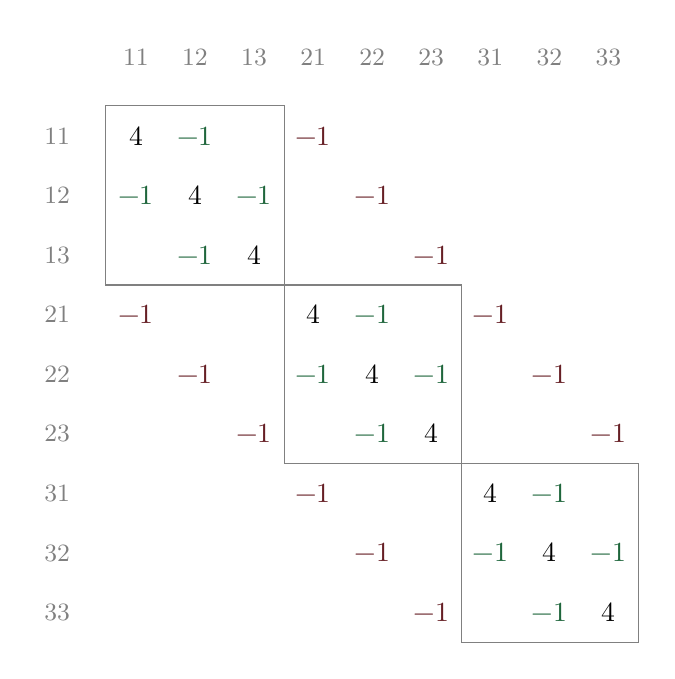
\begin{tikzpicture}
    \tikzstyle{every node}=[minimum size=0.75cm];
    \matrix(M) [matrix of math nodes]
    {
      4         & \greenone & \zeroel   & \redone   & \zeroel   & \zeroel   & \zeroel   & \zeroel   & \zeroel   \\
      \greenone & 4         & \greenone & \zeroel   & \redone   & \zeroel   & \zeroel   & \zeroel   & \zeroel   \\
      \zeroel   & \greenone & 4         & \zeroel   & \zeroel   & \redone   & \zeroel   & \zeroel   & \zeroel   \\
      \redone   & \zeroel   & \zeroel   & 4         & \greenone & \zeroel   & \redone   & \zeroel   & \zeroel   \\
      \zeroel   & \redone   & \zeroel   & \greenone & 4         & \greenone & \zeroel   & \redone   & \zeroel   \\
      \zeroel   & \zeroel   & \redone   & \zeroel   & \greenone & 4         & \zeroel   & \zeroel   & \redone   \\
      \zeroel   & \zeroel   & \zeroel   & \redone   & \zeroel   & \zeroel   & 4         & \greenone & \zeroel   \\
      \zeroel   & \zeroel   & \zeroel   & \zeroel   & \redone   & \zeroel   & \greenone & 4         & \greenone \\
      \zeroel   & \zeroel   & \zeroel   & \zeroel   & \zeroel   & \redone   & \zeroel   & \greenone & 4         \\
    };
    % Diag boxes
    \draw[gray] (M-1-1.north west) rectangle (M-3-3.south east);
    \draw[gray] (M-3-3.south east) rectangle (M-6-6.south east);
    \draw[gray] (M-6-6.south east) rectangle (M-9-9.south east);
    % position markers
    \node[gray, above of = M-1-1] {{\small 11}};
    \node[gray, above of = M-1-2] {{\small 12}};
    \node[gray, above of = M-1-3] {{\small 13}};
    \node[gray, above of = M-1-4] {{\small 21}};
    \node[gray, above of = M-1-5] {{\small 22}};
    \node[gray, above of = M-1-6] {{\small 23}};
    \node[gray, above of = M-1-7] {{\small 31}};
    \node[gray, above of = M-1-8] {{\small 32}};
    \node[gray, above of = M-1-9] {{\small 33}};

    \node[gray, left of = M-1-1] {{\small 11}};
    \node[gray, left of = M-2-1] {{\small 12}};
    \node[gray, left of = M-3-1] {{\small 13}};
    \node[gray, left of = M-4-1] {{\small 21}};
    \node[gray, left of = M-5-1] {{\small 22}};
    \node[gray, left of = M-6-1] {{\small 23}};
    \node[gray, left of = M-7-1] {{\small 31}};
    \node[gray, left of = M-8-1] {{\small 32}};
    \node[gray, left of = M-9-1] {{\small 33}};
  \end{tikzpicture}
\end{center}

The diagonal blocks are the same as in the 1D case. The first diagonal
of ones connect the elements $i,j$ of $Ψ$ with $i±1, j$ (terms $\textcolor{nicegreen}{Ψ_±}$
in the equation) whereas the
second one connects $i, j$ with $i, j±1$ (terms $\textcolor{nicered}{Ψ^±}$).\footnote{
  Remember that $Ψ(x,y)$ is a 1D vector, despite its intrinsic 2D nature.
}

In the 3D case, we have
$Ψ(\textcolor{nicegreen}{x}, \textcolor{nicered}{y},
\textcolor{niceblue}{z})$; the new dimension amounts only to add
another diagonal of ones:

\begin{center}
  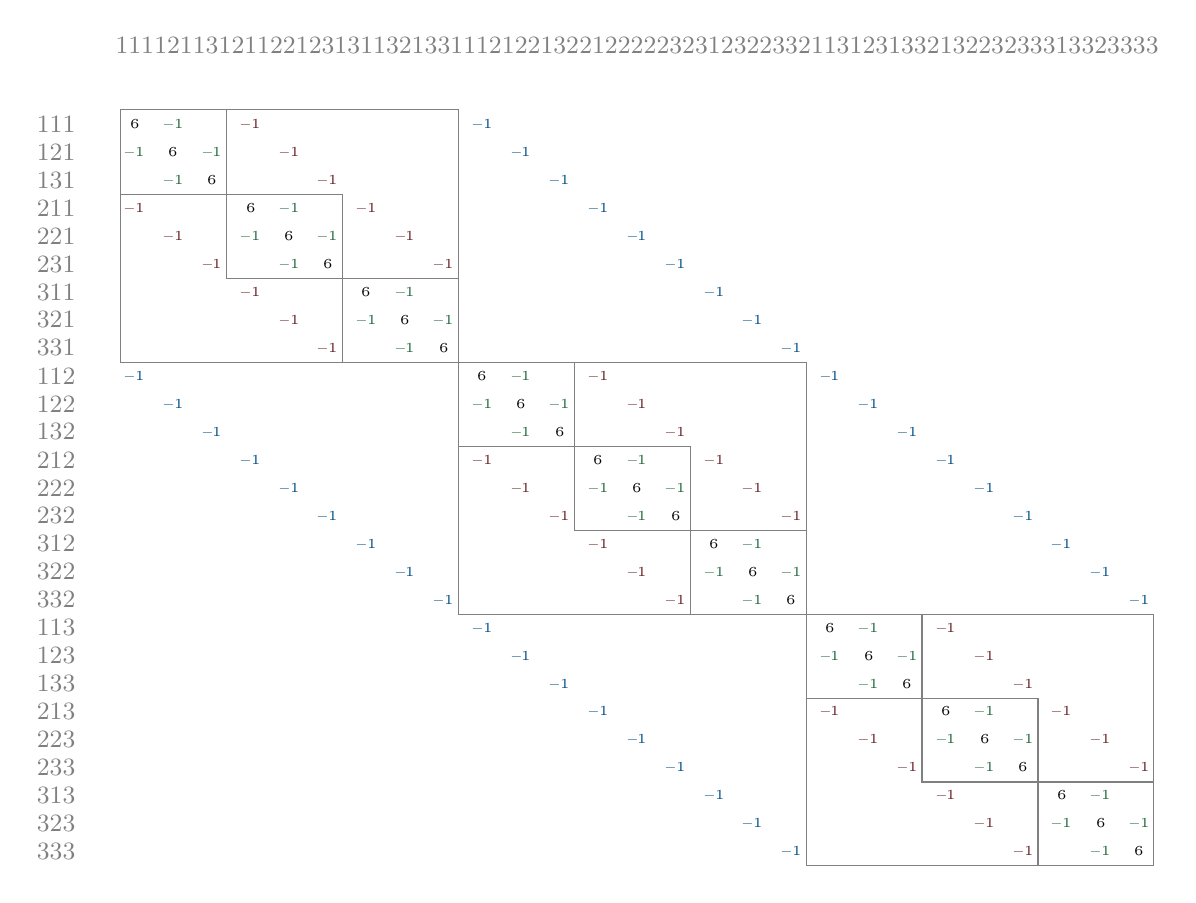
\begin{tikzpicture}
    \tikzstyle{every node}=[minimum size=0.25cm, font=\tiny];
    \matrix(M) [matrix of math nodes]
    {
      6         & \greenone & \zeroel   & \redone   & \zeroel   & \zeroel   & \zeroel   & \zeroel   & \zeroel   & \blueone  & \zeroel   & \zeroel   & \zeroel   & \zeroel   & \zeroel   & \zeroel   & \zeroel   & \zeroel   & \zeroel   & \zeroel   & \zeroel   & \zeroel   & \zeroel   & \zeroel   & \zeroel   & \zeroel   & \zeroel   \\
      \greenone & 6         & \greenone & \zeroel   & \redone   & \zeroel   & \zeroel   & \zeroel   & \zeroel   & \zeroel   & \blueone  & \zeroel   & \zeroel   & \zeroel   & \zeroel   & \zeroel   & \zeroel   & \zeroel   & \zeroel   & \zeroel   & \zeroel   & \zeroel   & \zeroel   & \zeroel   & \zeroel   & \zeroel   & \zeroel   \\
      \zeroel   & \greenone & 6         & \zeroel   & \zeroel   & \redone   & \zeroel   & \zeroel   & \zeroel   & \zeroel   & \zeroel   & \blueone  & \zeroel   & \zeroel   & \zeroel   & \zeroel   & \zeroel   & \zeroel   & \zeroel   & \zeroel   & \zeroel   & \zeroel   & \zeroel   & \zeroel   & \zeroel   & \zeroel   & \zeroel   \\
      \redone   & \zeroel   & \zeroel   & 6         & \greenone & \zeroel   & \redone   & \zeroel   & \zeroel   & \zeroel   & \zeroel   & \zeroel   & \blueone  & \zeroel   & \zeroel   & \zeroel   & \zeroel   & \zeroel   & \zeroel   & \zeroel   & \zeroel   & \zeroel   & \zeroel   & \zeroel   & \zeroel   & \zeroel   & \zeroel   \\
      \zeroel   & \redone   & \zeroel   & \greenone & 6         & \greenone & \zeroel   & \redone   & \zeroel   & \zeroel   & \zeroel   & \zeroel   & \zeroel   & \blueone  & \zeroel   & \zeroel   & \zeroel   & \zeroel   & \zeroel   & \zeroel   & \zeroel   & \zeroel   & \zeroel   & \zeroel   & \zeroel   & \zeroel   & \zeroel   \\
      \zeroel   & \zeroel   & \redone   & \zeroel   & \greenone & 6         & \zeroel   & \zeroel   & \redone   & \zeroel   & \zeroel   & \zeroel   & \zeroel   & \zeroel   & \blueone  & \zeroel   & \zeroel   & \zeroel   & \zeroel   & \zeroel   & \zeroel   & \zeroel   & \zeroel   & \zeroel   & \zeroel   & \zeroel   & \zeroel   \\
      \zeroel   & \zeroel   & \zeroel   & \redone   & \zeroel   & \zeroel   & 6         & \greenone & \zeroel   & \zeroel   & \zeroel   & \zeroel   & \zeroel   & \zeroel   & \zeroel   & \blueone  & \zeroel   & \zeroel   & \zeroel   & \zeroel   & \zeroel   & \zeroel   & \zeroel   & \zeroel   & \zeroel   & \zeroel   & \zeroel   \\
      \zeroel   & \zeroel   & \zeroel   & \zeroel   & \redone   & \zeroel   & \greenone & 6         & \greenone & \zeroel   & \zeroel   & \zeroel   & \zeroel   & \zeroel   & \zeroel   & \zeroel   & \blueone  & \zeroel   & \zeroel   & \zeroel   & \zeroel   & \zeroel   & \zeroel   & \zeroel   & \zeroel   & \zeroel   & \zeroel   \\
      \zeroel   & \zeroel   & \zeroel   & \zeroel   & \zeroel   & \redone   & \zeroel   & \greenone & 6         & \zeroel   & \zeroel   & \zeroel   & \zeroel   & \zeroel   & \zeroel   & \zeroel   & \zeroel   & \blueone  & \zeroel   & \zeroel   & \zeroel   & \zeroel   & \zeroel   & \zeroel   & \zeroel   & \zeroel   & \zeroel   \\
      \blueone  & \zeroel   & \zeroel   & \zeroel   & \zeroel   & \zeroel   & \zeroel   & \zeroel   & \zeroel   & 6         & \greenone & \zeroel   & \redone   & \zeroel   & \zeroel   & \zeroel   & \zeroel   & \zeroel   & \blueone  & \zeroel   & \zeroel   & \zeroel   & \zeroel   & \zeroel   & \zeroel   & \zeroel   & \zeroel   \\
      \zeroel   & \blueone  & \zeroel   & \zeroel   & \zeroel   & \zeroel   & \zeroel   & \zeroel   & \zeroel   & \greenone & 6         & \greenone & \zeroel   & \redone   & \zeroel   & \zeroel   & \zeroel   & \zeroel   & \zeroel   & \blueone  & \zeroel   & \zeroel   & \zeroel   & \zeroel   & \zeroel   & \zeroel   & \zeroel   \\
      \zeroel   & \zeroel   & \blueone  & \zeroel   & \zeroel   & \zeroel   & \zeroel   & \zeroel   & \zeroel   & \zeroel   & \greenone & 6         & \zeroel   & \zeroel   & \redone   & \zeroel   & \zeroel   & \zeroel   & \zeroel   & \zeroel   & \blueone  & \zeroel   & \zeroel   & \zeroel   & \zeroel   & \zeroel   & \zeroel   \\
      \zeroel   & \zeroel   & \zeroel   & \blueone  & \zeroel   & \zeroel   & \zeroel   & \zeroel   & \zeroel   & \redone   & \zeroel   & \zeroel   & 6         & \greenone & \zeroel   & \redone   & \zeroel   & \zeroel   & \zeroel   & \zeroel   & \zeroel   & \blueone  & \zeroel   & \zeroel   & \zeroel   & \zeroel   & \zeroel   \\
      \zeroel   & \zeroel   & \zeroel   & \zeroel   & \blueone  & \zeroel   & \zeroel   & \zeroel   & \zeroel   & \zeroel   & \redone   & \zeroel   & \greenone & 6         & \greenone & \zeroel   & \redone   & \zeroel   & \zeroel   & \zeroel   & \zeroel   & \zeroel   & \blueone  & \zeroel   & \zeroel   & \zeroel   & \zeroel   \\
      \zeroel   & \zeroel   & \zeroel   & \zeroel   & \zeroel   & \blueone  & \zeroel   & \zeroel   & \zeroel   & \zeroel   & \zeroel   & \redone   & \zeroel   & \greenone & 6         & \zeroel   & \zeroel   & \redone   & \zeroel   & \zeroel   & \zeroel   & \zeroel   & \zeroel   & \blueone  & \zeroel   & \zeroel   & \zeroel   \\
      \zeroel   & \zeroel   & \zeroel   & \zeroel   & \zeroel   & \zeroel   & \blueone  & \zeroel   & \zeroel   & \zeroel   & \zeroel   & \zeroel   & \redone   & \zeroel   & \zeroel   & 6         & \greenone & \zeroel   & \zeroel   & \zeroel   & \zeroel   & \zeroel   & \zeroel   & \zeroel   & \blueone  & \zeroel   & \zeroel   \\
      \zeroel   & \zeroel   & \zeroel   & \zeroel   & \zeroel   & \zeroel   & \zeroel   & \blueone  & \zeroel   & \zeroel   & \zeroel   & \zeroel   & \zeroel   & \redone   & \zeroel   & \greenone & 6         & \greenone & \zeroel   & \zeroel   & \zeroel   & \zeroel   & \zeroel   & \zeroel   & \zeroel   & \blueone  & \zeroel   \\
      \zeroel   & \zeroel   & \zeroel   & \zeroel   & \zeroel   & \zeroel   & \zeroel   & \zeroel   & \blueone  & \zeroel   & \zeroel   & \zeroel   & \zeroel   & \zeroel   & \redone   & \zeroel   & \greenone & 6         & \zeroel   & \zeroel   & \zeroel   & \zeroel   & \zeroel   & \zeroel   & \zeroel   & \zeroel   & \blueone  \\
      \zeroel   & \zeroel   & \zeroel   & \zeroel   & \zeroel   & \zeroel   & \zeroel   & \zeroel   & \zeroel   & \blueone  & \zeroel   & \zeroel   & \zeroel   & \zeroel   & \zeroel   & \zeroel   & \zeroel   & \zeroel   & 6         & \greenone & \zeroel   & \redone   & \zeroel   & \zeroel   & \zeroel   & \zeroel   & \zeroel   \\
      \zeroel   & \zeroel   & \zeroel   & \zeroel   & \zeroel   & \zeroel   & \zeroel   & \zeroel   & \zeroel   & \zeroel   & \blueone  & \zeroel   & \zeroel   & \zeroel   & \zeroel   & \zeroel   & \zeroel   & \zeroel   & \greenone & 6         & \greenone & \zeroel   & \redone   & \zeroel   & \zeroel   & \zeroel   & \zeroel   \\
      \zeroel   & \zeroel   & \zeroel   & \zeroel   & \zeroel   & \zeroel   & \zeroel   & \zeroel   & \zeroel   & \zeroel   & \zeroel   & \blueone  & \zeroel   & \zeroel   & \zeroel   & \zeroel   & \zeroel   & \zeroel   & \zeroel   & \greenone & 6         & \zeroel   & \zeroel   & \redone   & \zeroel   & \zeroel   & \zeroel   \\
      \zeroel   & \zeroel   & \zeroel   & \zeroel   & \zeroel   & \zeroel   & \zeroel   & \zeroel   & \zeroel   & \zeroel   & \zeroel   & \zeroel   & \blueone  & \zeroel   & \zeroel   & \zeroel   & \zeroel   & \zeroel   & \redone   & \zeroel   & \zeroel   & 6         & \greenone & \zeroel   & \redone   & \zeroel   & \zeroel   \\
      \zeroel   & \zeroel   & \zeroel   & \zeroel   & \zeroel   & \zeroel   & \zeroel   & \zeroel   & \zeroel   & \zeroel   & \zeroel   & \zeroel   & \zeroel   & \blueone  & \zeroel   & \zeroel   & \zeroel   & \zeroel   & \zeroel   & \redone   & \zeroel   & \greenone & 6         & \greenone & \zeroel   & \redone   & \zeroel   \\
      \zeroel   & \zeroel   & \zeroel   & \zeroel   & \zeroel   & \zeroel   & \zeroel   & \zeroel   & \zeroel   & \zeroel   & \zeroel   & \zeroel   & \zeroel   & \zeroel   & \blueone  & \zeroel   & \zeroel   & \zeroel   & \zeroel   & \zeroel   & \redone   & \zeroel   & \greenone & 6         & \zeroel   & \zeroel   & \redone   \\
      \zeroel   & \zeroel   & \zeroel   & \zeroel   & \zeroel   & \zeroel   & \zeroel   & \zeroel   & \zeroel   & \zeroel   & \zeroel   & \zeroel   & \zeroel   & \zeroel   & \zeroel   & \blueone  & \zeroel   & \zeroel   & \zeroel   & \zeroel   & \zeroel   & \redone   & \zeroel   & \zeroel   & 6         & \greenone & \zeroel   \\
      \zeroel   & \zeroel   & \zeroel   & \zeroel   & \zeroel   & \zeroel   & \zeroel   & \zeroel   & \zeroel   & \zeroel   & \zeroel   & \zeroel   & \zeroel   & \zeroel   & \zeroel   & \zeroel   & \blueone  & \zeroel   & \zeroel   & \zeroel   & \zeroel   & \zeroel   & \redone   & \zeroel   & \greenone & 6         & \greenone \\
      \zeroel   & \zeroel   & \zeroel   & \zeroel   & \zeroel   & \zeroel   & \zeroel   & \zeroel   & \zeroel   & \zeroel   & \zeroel   & \zeroel   & \zeroel   & \zeroel   & \zeroel   & \zeroel   & \zeroel   & \blueone  & \zeroel   & \zeroel   & \zeroel   & \zeroel   & \zeroel   & \redone   & \zeroel   & \greenone & 6         \\
    };
    % Diag boxes
    \draw[gray] (M-1-1.north west) rectangle (M-3-3.south east);
    \draw[gray] (M-3-3.south east) rectangle (M-6-6.south east);
    \draw[gray] (M-6-6.south east) rectangle (M-9-9.south east);
    \draw[gray] (M-9-9.south east) rectangle (M-12-12.south east);
    \draw[gray] (M-12-12.south east) rectangle (M-15-15.south east);
    \draw[gray] (M-15-15.south east) rectangle (M-18-18.south east);
    \draw[gray] (M-18-18.south east) rectangle (M-21-21.south east);
    \draw[gray] (M-21-21.south east) rectangle (M-24-24.south east);
    \draw[gray] (M-24-24.south east) rectangle (M-27-27.south east);

    % 3 block Diag boxes
    \draw[gray] (M-1-1.north west) rectangle (M-9-9.south east);
    \draw[gray] (M-9-9.south east) rectangle (M-18-18.south east);
    \draw[gray] (M-18-18.south east) rectangle (M-27-27.south east);

    % position markers
    \node[gray, above of = M-1-1] {{\small 111}};
    \node[gray, above of = M-1-2] {{\small 121}};
    \node[gray, above of = M-1-3] {{\small 131}};
    \node[gray, above of = M-1-4] {{\small 211}};
    \node[gray, above of = M-1-5] {{\small 221}};
    \node[gray, above of = M-1-6] {{\small 231}};
    \node[gray, above of = M-1-7] {{\small 311}};
    \node[gray, above of = M-1-8] {{\small 321}};
    \node[gray, above of = M-1-9] {{\small 331}};
    \node[gray, above of = M-1-10] {{\small 112}};
    \node[gray, above of = M-1-11] {{\small 122}};
    \node[gray, above of = M-1-12] {{\small 132}};
    \node[gray, above of = M-1-13] {{\small 212}};
    \node[gray, above of = M-1-14] {{\small 222}};
    \node[gray, above of = M-1-15] {{\small 232}};
    \node[gray, above of = M-1-16] {{\small 312}};
    \node[gray, above of = M-1-17] {{\small 322}};
    \node[gray, above of = M-1-18] {{\small 332}};
    \node[gray, above of = M-1-19] {{\small 113}};
    \node[gray, above of = M-1-20] {{\small 123}};
    \node[gray, above of = M-1-21] {{\small 133}};
    \node[gray, above of = M-1-22] {{\small 213}};
    \node[gray, above of = M-1-23] {{\small 223}};
    \node[gray, above of = M-1-24] {{\small 233}};
    \node[gray, above of = M-1-25] {{\small 313}};
    \node[gray, above of = M-1-26] {{\small 323}};
    \node[gray, above of = M-1-27] {{\small 333}};

    \node[gray, left of = M-1-1] {{\small 111}};
    \node[gray, left of = M-2-1] {{\small 121}};
    \node[gray, left of = M-3-1] {{\small 131}};
    \node[gray, left of = M-4-1] {{\small 211}};
    \node[gray, left of = M-5-1] {{\small 221}};
    \node[gray, left of = M-6-1] {{\small 231}};
    \node[gray, left of = M-7-1] {{\small 311}};
    \node[gray, left of = M-8-1] {{\small 321}};
    \node[gray, left of = M-9-1] {{\small 331}};
    \node[gray, left of = M-10-1] {{\small 112}};
    \node[gray, left of = M-11-1] {{\small 122}};
    \node[gray, left of = M-12-1] {{\small 132}};
    \node[gray, left of = M-13-1] {{\small 212}};
    \node[gray, left of = M-14-1] {{\small 222}};
    \node[gray, left of = M-15-1] {{\small 232}};
    \node[gray, left of = M-16-1] {{\small 312}};
    \node[gray, left of = M-17-1] {{\small 322}};
    \node[gray, left of = M-18-1] {{\small 332}};
    \node[gray, left of = M-19-1] {{\small 113}};
    \node[gray, left of = M-20-1] {{\small 123}};
    \node[gray, left of = M-21-1] {{\small 133}};
    \node[gray, left of = M-22-1] {{\small 213}};
    \node[gray, left of = M-23-1] {{\small 223}};
    \node[gray, left of = M-24-1] {{\small 233}};
    \node[gray, left of = M-25-1] {{\small 313}};
    \node[gray, left of = M-26-1] {{\small 323}};
    \node[gray, left of = M-27-1] {{\small 333}};
  \end{tikzpicture}
\end{center}

\bibliography{biblio}{}
\bibliographystyle{plain}

\end{document}
